\documentclass[journal, a4paper]{IEEEtran}

% some very useful LaTeX packages include:

%\usepackage{cite}      % Written by Donald Arseneau
                        % V1.6 and later of IEEEtran pre-defines the format
                        % of the cite.sty package \cite{} output to follow
                        % that of IEEE. Loading the cite package will
                        % result in citation numbers being automatically
                        % sorted and properly "ranged". i.e.,
                        % [1], [9], [2], [7], [5], [6]
                        % (without using cite.sty)
                        % will become:
                        % [1], [2], [5]--[7], [9] (using cite.sty)
                        % cite.sty's \cite will automatically add leading
                        % space, if needed. Use cite.sty's noadjust option
                        % (cite.sty V3.8 and later) if you want to turn this
                        % off. cite.sty is already installed on most LaTeX
                        % systems. The latest version can be obtained at:
                        % http://www.ctan.org/tex-archive/macros/latex/contrib/supported/cite/

\usepackage{graphicx}   % Written by David Carlisle and Sebastian Rahtz
                        % Required if you want graphics, photos, etc.
                        % graphicx.sty is already installed on most LaTeX
                        % systems. The latest version and documentation can
                        % be obtained at:
                        % http://www.ctan.org/tex-archive/macros/latex/required/graphics/
                        % Another good source of documentation is "Using
                        % Imported Graphics in LaTeX2e" by Keith Reckdahl
                        % which can be found as esplatex.ps and epslatex.pdf
                        % at: http://www.ctan.org/tex-archive/info/

%\usepackage{psfrag}    % Written by Craig Barratt, Michael C. Grant,
                        % and David Carlisle
                        % This package allows you to substitute LaTeX
                        % commands for text in imported EPS graphic files.
                        % In this way, LaTeX symbols can be placed into
                        % graphics that have been generated by other
                        % applications. You must use latex->dvips->ps2pdf
                        % workflow (not direct pdf output from pdflatex) if
                        % you wish to use this capability because it works
                        % via some PostScript tricks. Alternatively, the
                        % graphics could be processed as separate files via
                        % psfrag and dvips, then converted to PDF for
                        % inclusion in the main file which uses pdflatex.
                        % Docs are in "The PSfrag System" by Michael C. Grant
                        % and David Carlisle. There is also some information
                        % about using psfrag in "Using Imported Graphics in
                        % LaTeX2e" by Keith Reckdahl which documents the
                        % graphicx package (see above). The psfrag package
                        % and documentation can be obtained at:
                        % http://www.ctan.org/tex-archive/macros/latex/contrib/supported/psfrag/

%\usepackage{subfigure} % Written by Steven Douglas Cochran
                        % This package makes it easy to put subfigures
                        % in your figures. i.e., "figure 1a and 1b"
                        % Docs are in "Using Imported Graphics in LaTeX2e"
                        % by Keith Reckdahl which also documents the graphicx
                        % package (see above). subfigure.sty is already
                        % installed on most LaTeX systems. The latest version
                        % and documentation can be obtained at:
                        % http://www.ctan.org/tex-archive/macros/latex/contrib/supported/subfigure/

\usepackage{url}        % Written by Donald Arseneau
                        % Provides better support for handling and breaking
                        % URLs. url.sty is already installed on most LaTeX
                        % systems. The latest version can be obtained at:
                        % http://www.ctan.org/tex-archive/macros/latex/contrib/other/misc/
                        % Read the url.sty source comments for usage information.

%\usepackage{stfloats}  % Written by Sigitas Tolusis
                        % Gives LaTeX2e the ability to do double column
                        % floats at the bottom of the page as well as the top.
                        % (e.g., "\begin{figure*}[!b]" is not normally
                        % possible in LaTeX2e). This is an invasive package
                        % which rewrites many portions of the LaTeX2e output
                        % routines. It may not work with other packages that
                        % modify the LaTeX2e output routine and/or with other
                        % versions of LaTeX. The latest version and
                        % documentation can be obtained at:
                        % http://www.ctan.org/tex-archive/macros/latex/contrib/supported/sttools/
                        % Documentation is contained in the stfloats.sty
                        % comments as well as in the presfull.pdf file.
                        % Do not use the stfloats baselinefloat ability as
                        % IEEE does not allow \baselineskip to stretch.
                        % Authors submitting work to the IEEE should note
                        % that IEEE rarely uses double column equations and
                        % that authors should try to avoid such use.
                        % Do not be tempted to use the cuted.sty or
                        % midfloat.sty package (by the same author) as IEEE
                        % does not format its papers in such ways.

\usepackage{amsmath}    % From the American Mathematical Society
                        % A popular package that provides many helpful commands
                        % for dealing with mathematics. Note that the AMSmath
                        % package sets \interdisplaylinepenalty to 10000 thus
                        % preventing page breaks from occurring within multiline
                        % equations. Use:
%\interdisplaylinepenalty=2500
                        % after loading amsmath to restore such page breaks
                        % as IEEEtran.cls normally does. amsmath.sty is already
                        % installed on most LaTeX systems. The latest version
                        % and documentation can be obtained at:
                        % http://www.ctan.org/tex-archive/macros/latex/required/amslatex/math/



% Other popular packages for formatting tables and equations include:

%\usepackage{array}
% Frank Mittelbach's and David Carlisle's array.sty which improves the
% LaTeX2e array and tabular environments to provide better appearances and
% additional user controls. array.sty is already installed on most systems.
% The latest version and documentation can be obtained at:
% http://www.ctan.org/tex-archive/macros/latex/required/tools/

% V1.6 of IEEEtran contains the IEEEeqnarray family of commands that can
% be used to generate multiline equations as well as matrices, tables, etc.

% Also of notable interest:
% Scott Pakin's eqparbox package for creating (automatically sized) equal
% width boxes. Available:
% http://www.ctan.org/tex-archive/macros/latex/contrib/supported/eqparbox/

% *** Do not adjust lengths that control margins, column widths, etc. ***
% *** Do not use packages that alter fonts (such as pslatex).         ***
% There should be no need to do such things with IEEEtran.cls V1.6 and later.


% Your document starts here!
\begin{document}
\begin{titlepage}

\newcommand{\HRule}{\rule{\linewidth}{0.5mm}} % Defines a new command for the horizontal lines, change thickness here

\center % Center everything on the page
 %----------------------------------------------------------------------------------------
%	LOGO SECTION
%----------------------------------------------------------------------------------------

~\\[1cm]

\includegraphics{SCUT.png}\\[2cm] % Include a department/university logo - this will require the graphicx package

%----------------------------------------------------------------------------------------
%	TITLE SECTION
%----------------------------------------------------------------------------------------

\HRule \\[1cm]
{ \huge \bfseries The Experiment Report of \textit{Machine Learning} }\\[0.6cm] % Title of your document
\HRule \\[2cm]
%----------------------------------------------------------------------------------------
%	HEADING SECTIONS
%----------------------------------------------------------------------------------------


\textsc{\LARGE \textbf{School:} School of Software Engineering}\\[1cm]
\textsc{\LARGE \textbf{Subject:} Software Engineering}\\[2cm]


%----------------------------------------------------------------------------------------
%	AUTHOR SECTION
%----------------------------------------------------------------------------------------

\begin{minipage}{0.4\textwidth}
\begin{flushleft} \large
\emph{Author:}\\
Da Ren % Your name
\end{flushleft}
\end{minipage}
~
\begin{minipage}{0.4\textwidth}
\begin{flushright} \large
\emph{Supervisor:} \\
Qingyao Wu % Supervisor's Name
\end{flushright}
\end{minipage}\\[2cm]
~
\begin{minipage}{0.4\textwidth}
\begin{flushleft} \large
\emph{Student ID:}\\
201720144900
\end{flushleft}
\end{minipage}
~
\begin{minipage}{0.4\textwidth}
\begin{flushright} \large
\emph{Grade:} \\
Graduate
\end{flushright}
\end{minipage}\\[2cm]

% If you don't want a supervisor, uncomment the two lines below and remove the section above
%\Large \emph{Author:}\\
%John \textsc{Smith}\\[3cm] % Your name

%----------------------------------------------------------------------------------------
%	DATE SECTION
%----------------------------------------------------------------------------------------

{\large \today}\\[2cm] % Date, change the \today to a set date if you want to be precise


%----------------------------------------------------------------------------------------

\vfill % Fill the rest of the page with whitespace

\end{titlepage}

% Define document title and author
	\title{Logistic Regression, Linear Classification and Stochastic Gradient Descent}
	\maketitle

% Write abstract here
\begin{abstract}
Gradient descent plays an important role in machine learning. It can help us get the optimal value of a function. However, one of the most important task in machine learning is to get the optimal value for loss function. Gradient descent is widely used in this task. However, people gradually find that traditional gradient descent performs not well when dealing with some tasks. Therefore, there are many modified gradient descent methods which are proposed. I implement NAG, RMSProp, AdaDelta and Adam in logistic regression and linear regression in this experiment.
\end{abstract}

% Each section begins with a \section{title} command
\section{Introduction}
	% \PARstart{}{} creates a tall first letter for this first paragraph
\PARstart{G}{radient} descent is a important method in machine learning. The most important tasks in many machine learning models is to update or calculate their parameters which can lead the corresponding loss functions value to be minimal value. Although gradient descent is widely used, researchers find that it has its own limitation. Therefore, there are many modified gradient descent methods which are proposed, \emph{e.g}. NAG, RMSProp, AdaDelta and Adam. In this experiment, I implement logistic regression and linear classification. And I use different methods to optimize their loss functions. My experiments' results show that all of them can optimize the models. However, their speed may be different.

% Main Part
\section{Methods and Theory}
Gradient descent is flexible since it can be easily used in different kinds of loss function. It is based on the observation that if the multi-variable function $F(x)$ is defined and differentiable in a neighborhood of a point $a$, then $F(x)$ decreases fastest if one goes from $a$ in the direction of the negative gradient of $F$ at $a$. Therefore, if we want to minimize the value of $F(x)$, we can move $a$ against the gradient of $F$. Therefore, $a$ can be updated by Eq.~\eqref{eq1}.
\begin{equation}
a_{t+1}=a_{t} + \lambda \Delta F(a_{t}) \label{eq1}
\end{equation}
where $a_{t}$ is the value of $a$ at time $t$, $\lambda$ is the learning rate which is always set to be a small value like 0.1. $\Delta F(a_{t})$ is the gradient value of $F(a_{t})$.

There are two experiments in my work. One is logistic regression, the other is linear classification. Therefore I have to choose different loss function to different tasks.

Logistic regression is a function that its output is limited from 0 to 1. It can be calculated as following:
\begin{equation}
y' = 1/(1+e^{-z}) \label{eq2}
\end{equation}
where
\begin{equation}
z = W^TX+b \label{eq3}
\end{equation}
where $W$ is the weight matrix and $b$ is the bias variable. However, we can add 1 at the end of $X$ so that the weight of the last column can act at the bias variable. Note $X'$ to be the features which is add 1 at the last column. We can calculate $z$ as following:
 \begin{equation}
z = W^TX' \label{eq4}
\end{equation}

To train the logistic regression, I choose log-likehood function as my loss function. It can be calculated by Eq.~\eqref{eq5}
\begin{equation}
L_1 = -1/n[\sum_{i=1}^ny_ilog h_w(x_i) + (1-y_i)log(1-h_w(x_i))] \label{eq5}
\end{equation}
where
\begin{equation}
h_w(X) = 1/(1+e^{-W^TX}) \label{eq6}
\end{equation}
In Eq.~\eqref{eq5}, $n$ is the total number of data and $y_i$ is the target value of data. The next step is to calculate the derivation of Eq.~\eqref{eq5}. The calculation process is in the following:
\begin{equation}
\begin{aligned}
\Delta L_1 / \Delta w & = -y*1/h_w(X)*{\Delta h_w(X)}/{\Delta W} + \\
& \quad \ (1-y)*1/(1-h_w(X))*{\Delta h_w(X)}/{\Delta W} \\
& =(h_w(X)-y)X
\label{eq7}
\end{aligned}
\end{equation}

After we get the the derivation of Eq.~\eqref{eq6}, we can calculate the gradient according to Eq.~\eqref{eq7} and update weight matrix according Eq.~\eqref{eq1}

In the linear classification task, I use the Eq.~\eqref{eq8} to calculate output.
\begin{equation}
y' = W^TX' \label{eq8}
\end{equation}

Since the function is different, I choose another loss function. The loss function I choose is called hinge loss, which can be described in Eq.~\eqref{eq9}
\begin{equation}
L_2 = \begin{Vmatrix}W\end{Vmatrix}^2/2 + C/m \sum_{i=1}^m max(0, 1-y_i(W^Tx_i+b))
\label{eq9}
\end{equation}
where $C$ is a hyperparameter which can be adjusted in different dataset.

To use the gradient descent to optimize the weight matrix, we have to calculate the the derivation of Eq.~\eqref{eq9}.
\begin{equation}
\Delta L_2 / \Delta w = W + C/m\sum_{i=1}^m g_w(x_i)
\label{eq10}
\end{equation}
where
\begin{equation}
g_w(x_i)=\begin{cases}
-y_ix_i\quad 1-y_i(W^Tx'_i) \geq 0 \\
0\quad \quad \quad 1-y_i(W^Tx'_i) < 0 \\
\end{cases}
\label{eq11}
\end{equation}

We can update the linear classification according to Eq.~\eqref{eq1} and use Eq.~\eqref{eq11} to calculate the gradient.

In this experiment, I not only used traditional gradient descent to train the models, but also use modified gradient descent. Their introduction is in the following.

Nesterov accelerated gradient(NAG) is a method which considers momentum. It can be calculated as following:
\begin{equation}
g_t=\Delta L(W_{t-1} - \gamma v_{t-1}) \label{eq12}
\end{equation}
\begin{equation}
v_t = \gamma v_{t-1} + \eta g_t \label{eq13}
\end{equation}
\begin{equation}
W_t = W_{t-1} - v_t \label{eq14}
\end{equation}
where $\gamma$ and $\eta$ are hyperparameters which can be set to be 0.9 and 0.1 respectively. $\eta$ is treated as the learning rate which is mentioned in Eq.~\eqref{eq1}.

RMSProp is a method which can solve the problem of AdaGrad that the learning rate tends to be 0. It can be calculated as following:
\begin{equation}
g_t=\Delta L(W_{t-1}) \label{eq15}
\end{equation}
\begin{equation}
G_t = \gamma G_{t-1} + (1-\gamma)g_t^2 \label{eq16}
\end{equation}
\begin{equation}
W_t = W_{t-1} - (\eta / \sqrt{G_t+\epsilon}) * g_t \label{eq17}
\end{equation}

AdaDelta is a special method that we don't need to set the learning rate. It can be calculated as following:
\begin{equation}
g_t=\Delta L(W_{t-1}) \label{eq18}
\end{equation}
\begin{equation}
G_t = \gamma G_{t-1} + (1-\gamma)g_t^2 \label{eq19}
\end{equation}
\begin{equation}
\Delta weight = -(\sqrt{\Delta_{t-1} + \epsilon}) / (\sqrt{G_{t} + \epsilon}) * g_t \label{eq20}
\end{equation}
\begin{equation}
weight = weight + \Delta weight \label{eq21}
\end{equation}
\begin{equation}
\Delta_{t}=\gamma \Delta_{t-1} + (1-\gamma)\Delta weight^2 \label{eq22}
\end{equation}

Adaptive estimates of lower-order moments (Adam) can be calculated as:
\begin{equation}
g_t=\Delta L(W_{t-1}) \label{eq23}
\end{equation}
\begin{equation}
m_t=\beta_1 \cdot m_{t-1} + (1-\beta_1) \cdot g_t \label{eq24}
\end{equation}
\begin{equation}
v_t=\beta_2 \cdot v_{t-1} + (1-\beta_2) \cdot g_t^2 \label{eq25}
\end{equation}
\begin{equation}
m'_t=m_t/(1-\beta_1^t) \label{eq26}
\end{equation}
\begin{equation}
v'_t=v_t/(1-\beta_2^t) \label{eq27}
\end{equation}
\begin{equation}
weight = weight - \eta m'_t / (\sqrt{v'_t+\epsilon})
\end{equation}
where $t$ is initialized to be 0 and add 1 at the beginning of each iterations.

After choosing the loss function and calculating their corresponding derivation, I can use different kinds of gradient descent to train these two models. When I calculate the gradient descent in this experiments, I don't use all of data. I randomly choose some of them to calculate the gradient. My experiment will be described in following.

\section{Experiments}
There will be two experiments which will be introduced. One is training the logistic regression and the other is training the linear classification. Both of them is trained in different kinds of gradient descent.

\subsection{Dataset}
I use a9a dataset in LIBSVM Data to train and test this two models. There are 32561 data in training set and 16281 data in test set. Each of them has 123 attributes.

\subsection{Implementation}
In this section, I will introduce the logistic regression experiment and linear classification experiment in detail.

There are different kinds of gradient descent in this experiment, the parameters I used is in the following.

\paragraph{Traditional Gradient Descent} Learning rate $a$ is set to be 0.1, and I will choose 20\% of training data randomly to train at each iterations.

\paragraph{NAG} Learning rate $\eta$ is set to be 0.1, and I will choose 20\% of training data randomly to train at each iterations. $\gamma$ is set to be 0.9.

\paragraph{RMSProp} Learning rate $\eta$ is set to be 0.02and I will choose 20\% of training data randomly to train at each iterations. $\gamma$ is set to be 0.9 and $\epsilon$ is set to be 1e-8.

\paragraph{AdaDelta} $\gamma$ is set to be 0.95 and $\epsilon$ is set to be 1e-6. I will choose 20\% of training data randomly to train at each iterations.

\paragraph{Adam} Learning rate $\eta$ is set to be 0.01. $\beta_1$ is set to be 0.999 $\beta_2$ is set to be 0.999 and $\epsilon$ is set to be 0.001. I will choose 20\% of training data randomly to train at each iterations.

The weight matrix in my experiments is initialized randomly. The other parameters which will be update at each iterations is initialized to be 0.

Before training in logistic regression model, I set all the -1 label to 0 label. It can help me apply the formula of logistic regression into this dataset easily. The iteration's number is set to 500. The loss value of test set is described in Fig.~\ref{fig_1}.
\begin{figure}[htbp]
\centerline{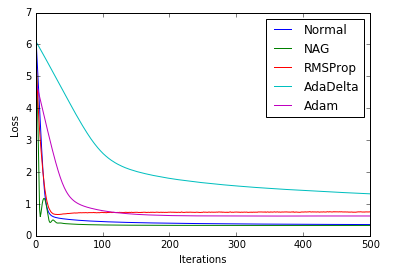
\includegraphics[height=150px]{line_1.png}}
\caption{The loss value of test set in logistic regression.}
\label{fig_1}
\end{figure}

In the linear classfication experiment, the parameters is set to be the same with the logistic regression. The loss value of test set is described in Fig.~\ref{fig_2}.

\begin{figure}[htbp]
\centerline{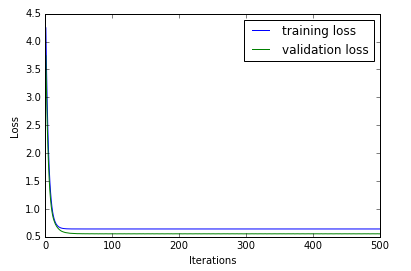
\includegraphics[height=150px]{line_2.png}}
\caption{The loss value of test set in linear classification.}
\label{fig_2}
\end{figure}

We can find that both of the loss value of training set and test set decrease quickly at the beginning and close to unchange at the end of iterations. It means that the value of loss function is closed to minimal value. However, logistic regression can get a smaller value than linear classification. And logistic regression performs more stable since the curve of classification which is update by RMSProp is not smooth. In Fig.~\ref{fig_1} and Fig.~\ref{fig_2}, we can find that Nag and RMSProp always optimize very fast.

After finish training, I set a threshold to classify the data in test set. I set the threshold to be 0.5 in logistic regression model, if the value calculated by model is smaller than 0.5, the corresponding data will be classified into one class (the label of this class is 0). If the value is larger or equal than 0.5, the corresponding data will be classified into another class (the label of this class is 1). The threshold in linear classification is 0, and the label is -1 and 1 respectively. And then I calculate the precision, recall and f1-score which is shown in Table~\ref{table_1} and Table~\ref{table_2}.

    \begin{table}[!hbt]
		% Center the table
		\begin{center}
		% Title of the table
		\caption{Classification Results in Logistic Regression}
		\label{table_1}
		% Table itself: here we have two columns which are centered and have lines to the left, right and in the middle: |c|c|
		\begin{tabular}{|c|c|c|c|c|}
			% To create a horizontal line, type \hline
			\hline
			% To end a column type &
			% For a linebreak type \\
			gradient descent  & precision & recall & f1-score & support \\
			\hline
			Traditional & 0.84 & 0.79 & 0.80  & 16281 \\
			\hline
			NAG & 0.85 & 0.71 & 0.73  & 16281 \\
			\hline
			RMSProp & 0.58 & 0.76 & 0.66 & 16281 \\
			\hline
            AdaDelta & 0.58 & 0.76 & 0.66 & 16281 \\
			\hline
            Adam & 0.58 & 0.76 & 0.66 & 16281 \\
			\hline
		\end{tabular}
		\end{center}
	\end{table}

    \begin{table}[!hbt]
		% Center the table
		\begin{center}
		% Title of the table
		\caption{Classification Results in Linear Classification}
		\label{table_2}
		% Table itself: here we have two columns which are centered and have lines to the left, right and in the middle: |c|c|
		\begin{tabular}{|c|c|c|c|c|}
			% To create a horizontal line, type \hline
			\hline
			% To end a column type &
			% For a linebreak type \\
			gradient descent  & precision & recall & f1-score & support \\
			\hline
			Traditional & 0.58 & 0.76 & 0.66 & 16281 \\
			\hline
			NAG & 0.58 & 0.76 & 0.66  & 16281 \\
			\hline
			RMSProp & 0.82 & 0.76 & 0.77 & 16281 \\
			\hline
            AdaDelta & 0.58 & 0.76 & 0.66 & 16281 \\
			\hline
            Adam & 0.58 & 0.76 & 0.66 & 16281 \\
			\hline
		\end{tabular}
		\end{center}
	\end{table}

From Table~\ref{table_1}, we can find that the traditional gradient descent and NAG get a better result than the other in logistic regression. I consider that it may be the problems from hyperparameters. I don't adjust a good value for all of the methods. However, we can find that the result in Table~\ref{table_2} is a bit different in Table~\ref{table_1}. Some methods perform quite different in two models. I consider that the hyperparameters which is suitable to one model may not be also suitable to other models.

\section{Conclusion}
In this experiment, I implement gradient descent in logistic regression and linear classification. And I use different kinds of gradient descent to optimize the models. I find that the hyperparameters play important roles in models. Hyperparameters will influence the result directly. And the results of two models also show that the hyperparameters which are suitable to one model may not suitable to other models. How to set a proper hyperparameters to models is an important problem. Different gradient descent methods can lead different curves of the same loss function. It means that each of them may be suitable for different kinds of data. 

% Your document ends here!
\end{document}
